\documentclass{beamer}

\mode<presentation> 
{
    \usetheme{Madrid}
}

\usepackage[utf8x]{inputenc}
\usepackage[english,russian]{babel}
\usepackage[T2A]{fontenc}
\usepackage{graphicx}
\usepackage{booktabs} 
\usepackage{mathtools}
\usepackage{amsmath}
\usepackage{wasysym}
\usepackage{subfig}
\usepackage{hyperref}
\usepackage{ulem}
\usepackage{ragged2e}
\usepackage{algorithm2e}
\usepackage{minted}

\usemintedstyle{borland}

\usefonttheme[onlymath]{serif}

\hypersetup
{
    colorlinks=true,
    linkcolor=white, 
    urlcolor=cyan
}

\title[Лекция 2]
{
    Лекция 2: 2-D цифровая фильтрация и операторы условного перехода в языке Си 
} 


\author[Д. А. Караваев]{Д. А. Караваев}

\institute[СПбГУТ] 
{
    Санкт-Петербургский государственный университет телекоммуникаций \\ им. проф. М. А. Бонч-Бруевича \\ 
    \vspace{0.2cm}
    Факультет РТС, Кафедра РОС \\
    \vspace{0.2cm}
    Факультатив <<Программирование в ЦОС>> \\
    \vspace{0.2cm}
    Осень 2019
}

\date[21.10.2019]{21.10.2019 Санкт-Петербург} 

\begin{document}
    \begin{frame}
        \titlepage 
    \end{frame}
    \begin{frame}
        \frametitle{Цифровая обработка изображений}
        \justifying
        {\bf Определение}: 
        \par
        {\it Двумерный сигнал} $x[n, m]$ - последовательность пронумерованная двумя индексами $(n, m)$. Значения $x[n, m]$ и $(n, m)$ могут иметь смысл интесивностии и пространственных индексов соответственно, тогда $x[n, m]$ есть {\it изображение}.
        \vspace{0.5cm}
        \par
        {\bf КИХ-фильтрация}: 
        \par
        Осуществляется через {\it двумерную (пространственную) свёртку}:
        \begin{equation}
            y[n, m] = \sum_{i = 0}^{T_{h} - 1}\sum_{j = 0}^{T_{w} - 1}h[i, j]x[n - i, m - j],
        \end{equation}
        где $x[n, m]$ - входной сигнал $(N_{h}, N_{w})$, $h[n, m]$ - ИХ размера $(T_{h}, T_{w})$ и
        $y[n, m]$ - выходной сигнал $(N_{h}, N_{w})$.
    \end{frame} 
    \begin{frame}
        \frametitle{Пример результата 2D КИХ-фильтрации}
        \begin{figure}[!tbp]
           \centering
           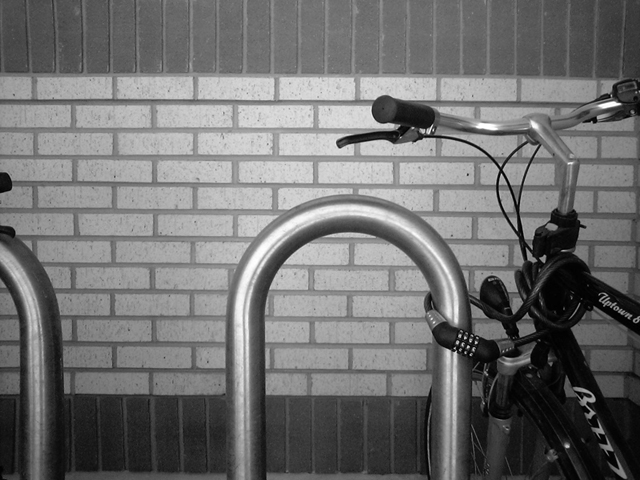
\includegraphics[width=0.5\textwidth]{pics/example_orig.jpg}
           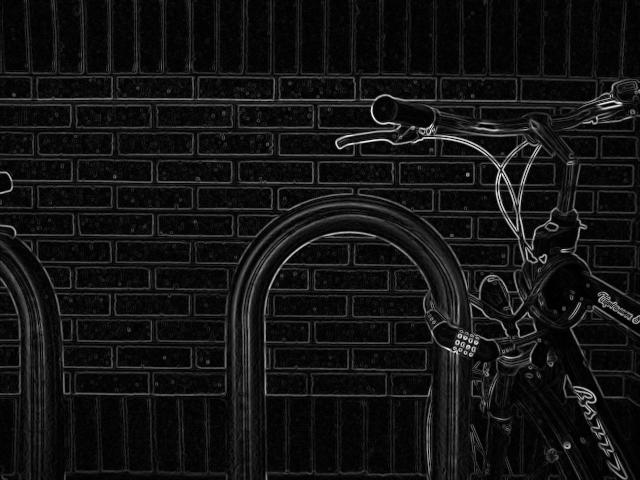
\includegraphics[width=0.5\textwidth]{pics/example_filt.jpg}
           \captionsetup{justification=centering}
           \captionof{figure}{Результат применения оператора Собеля \\ (\url{https://en.wikipedia.org/wiki/Sobel_operator}).}
       \end{figure}
    \end{frame}
    \begin{frame}
        \frametitle{Схема 2D свёртки}
        \begin{figure}[!tbp]
           \centering
           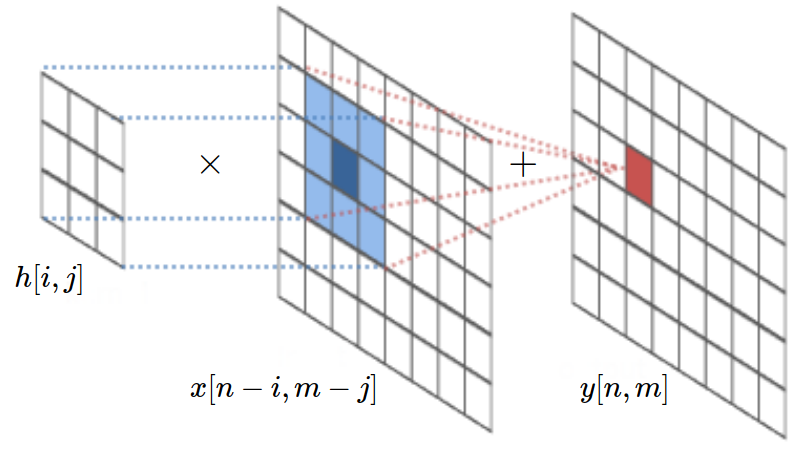
\includegraphics[width=\textwidth]{pics/2Dconv.png}
       \end{figure}
    \end{frame}
    \begin{frame}[fragile]
        \frametitle{Граничный случай (дополнение нулями)}
        \justifying
        {\bf Замечание}: В этот раз мы прибегнем к {\it неявному} дополнению нулями, проверяя условие выхода за границы сигнала. 
        Для этого нужна конструкция {\it условного перехода} (a.k.a {\texttt{if-else}}).
        \begin{figure}[!tbp]
            \centering
            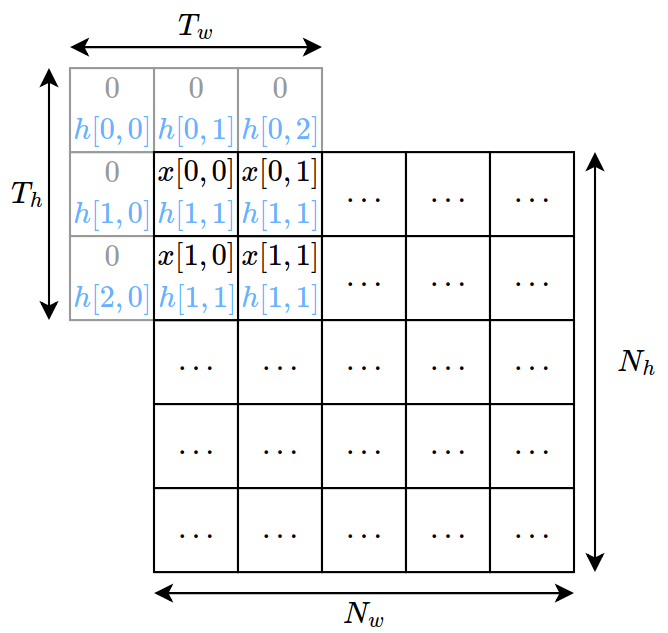
\includegraphics[width=0.55\textwidth]{pics/border.png}
        \end{figure}
    \end{frame}
    \begin{frame}{Псевдокод алгоритма 2D свёртки}
        \begin{algorithm}[H]
            \SetKwInOut{Input}{Вход}
            \SetKwInOut{Output}{Выход}
            \Input{$x[n, m]$ - размера $(N_{h}, N_{w})$, $h[n, m]$ - размера $(T_{h}, T_{w})$.}
            \Output{$y[n, m]$ - размера $(N_{h}, N_{w})$.}
            \BlankLine
            \For{$n \leftarrow 0$ \KwTo $N_{h} - 1$} 
            {
                \For{$m \leftarrow 0$ \KwTo $N_{w} - 1$} 
                {
                    $y[n, m] \leftarrow 0$
                    \par
                    \For{$i\leftarrow 0$ \KwTo $T_{h} - 1$}
                    {
                        \For{$j\leftarrow 0$ \KwTo $T_{w} - 1$}
                        {
                            \If{$(n - i) \geq 0 \wedge (m - j) \geq 0$}
                            {
                                 $y[n, m] \leftarrow y[n, m] + h[i, j]x[n - i, m- j]$
                            }
                        }
                    }
                }
            }
        \end{algorithm}
        \par
        \justifying
        {\bf Замечание:} Как в языке Си реализовать логические выражения и условный переход?
    \end{frame}
    \begin{frame}[fragile]{Логические выражения в Си}
        \begin{minted}[frame=lines,        framesep=2mm,
                       baselinestretch=1.2, fontsize=\footnotesize,
                       linenos]{c}
/* Некоторые переменные: */
float x = 1.0;
float y = -54.12;
float z = -4.12;
/* Логические выражения - выражения, значения которых true/false.*/
/* Состоят из комбинации операций сравнения: (==, !=, <=, >=, <, >) и */
/* логических операций (и, или и не): */
int predicat0 = (x < y) && (x > 0); /* (x < y) и (x > 0).*/
int predicat1 = ((x + 10) < y) || (y > 100); /* (x < y) или (x > 0).*/
int not_predicat0 = !predicat0; /* Значение противоположеное predicat0.*/
/* В языке Си есть тип для хранения результата лог. выражения: bool */
bool truth = (x <= 0) || (x > 0);
/* У операций (и, или и не) есть свой порядок действий, */
/* как у *, + и - соответственно: */
bool example = ((x > 3.14) && (y == 2 * 3.14)) || !(z >= -5);
        \end{minted}
    \end{frame}
    \begin{frame}[fragile]{Оператор условного перехода в Си}
        \begin{minted}[frame=lines,        framesep=2mm,
                       baselinestretch=1.2, fontsize=\footnotesize,
                       linenos]{c}
/* Всё стандартным образом: */
if (/* какое-то логическое выражение */)
{
    /* если выражение истинно исполняется код тут. */
}
else
{
    /* если выражение ложно исполняется код тут. */
}
/* Можно делать так: */
if (/* какое-то логическое выражение */)
{
    /* если выражение истинно исполняется код тут. */
}
/* Без кода на противоположное условие.*/
        \end{minted}
    \end{frame}
    \begin{frame}[fragile]{Множественный условный переход в Си}
        \begin{minted}[frame=lines,        framesep=2mm,
                       baselinestretch=1.2, fontsize=\footnotesize,
                       linenos]{c}
/* Оператор множественного условного перехода удобен для 
 * проверки нескольких выражений: */
if (/* какое-то логическое выражение_0*/)
{
    /* если выражение_0 истинно исполняется код тут. */
}
else if (/* какое-то логическое выражение 1*/)
{
    /* если выражение_1 ложно исполняется код тут. */
}
/* ... */
else
{
    /* если никакое выражние_(0, 1 ...) неистинно исполняется код тут. */
}
        \end{minted}
    \end{frame}
    \begin{frame}[fragile]{Пример условного перехода в Си}
        \begin{minted}[frame=lines,        framesep=2mm,
                       baselinestretch=1.2, fontsize=\footnotesize,
                       linenos]{c}
float x = 4.2;
float y = -4.3;
float z = 0.0;
if (x >= y) /* Проверяем выражение: */
{
    z = x + y;
}
else /* иначе: */
{
    z = x * y;
} /* или так: */
if ((x > 0) && (y < 0))
{
    z = x / y; /* Если выражение неверно, то z останется равным 0. */
}
        \end{minted}
    \end{frame}
    \begin{frame}[fragile]{Представление изображения в компьютере (Си)}
        \begin{minted}[frame=lines,        framesep=2mm,
                       baselinestretch=1.2, fontsize=\footnotesize,
                       linenos]{c}
/* В Си изображение (ЧБ) можно интерпретировать как двумерныме массивы
 * типа uint8_t (интенсивность белого): */
typedef unsigned char uint8_t; /* [0, 255]. */
/* !Внимание велик риск переполнения! */
uint8_t x[100][100]; /* Массив 100 на 100. */
x[10][25] = 24; /* Элемент (отсчёт) в 11 строке и в 26 столбце == 24. */
/* Будем использовать указатели по причине нефиксированного размера: */
uint8_t** y = x; /* Инициализируем указатель на двумерный массив. */
for (size_t n = 0; n < 100; n++) /* По строкам: */
{
    for (size_t m = 0; m < 100; m++) /* По столбцам: */
    {
        y[n][m] = 34; /* (n-ый, m-ый) элемент (пиксель). */
    }
}
        \end{minted}
    \end{frame}
    \begin{frame}
        \frametitle{Иллюстрация двойного указателя}
        \begin{figure}[!tbp]
           \centering
           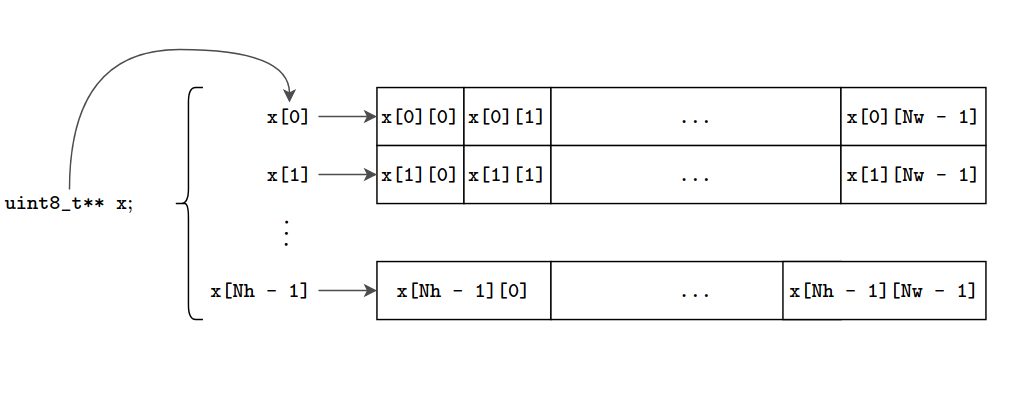
\includegraphics[width=\textwidth]{pics/2Dptrs.png}
       \end{figure}
    \end{frame}
    \begin{frame}[fragile]{Прототип функции}
        \begin{minted}[frame=lines,        framesep=2mm,
                       baselinestretch=1.2, fontsize=\footnotesize,
                       linenos]{c}
/*!
 * \param[in] x - 2-мерный входной сигнал.
 * \param[out] y - 2-мерный выходной сигнал.
 * \param[in] Nh - высота входного сигнала.
 * \param[in] Nw - ширина входного сигнала.
 * \param[in] h - ИХ.
 * \param[in] Th - высота ИХ.
 * \param[in] Th - ширина ИХ.
 * \return 0 - успех, -1 - не реализована.
 */
int DSP_convolve_2D(const uint8_t** x, uint8_t** y, size_t Nh, size_t Nw, 
                    const int8_t**  h, size_t Th,  size_t Tw)
{
    return -1;
}
        \end{minted}
    \end{frame}
    \begin{frame}[fragile]
        \frametitle{Результат 2D свёртки}
        \begin{figure}[!tbp]
           \centering
           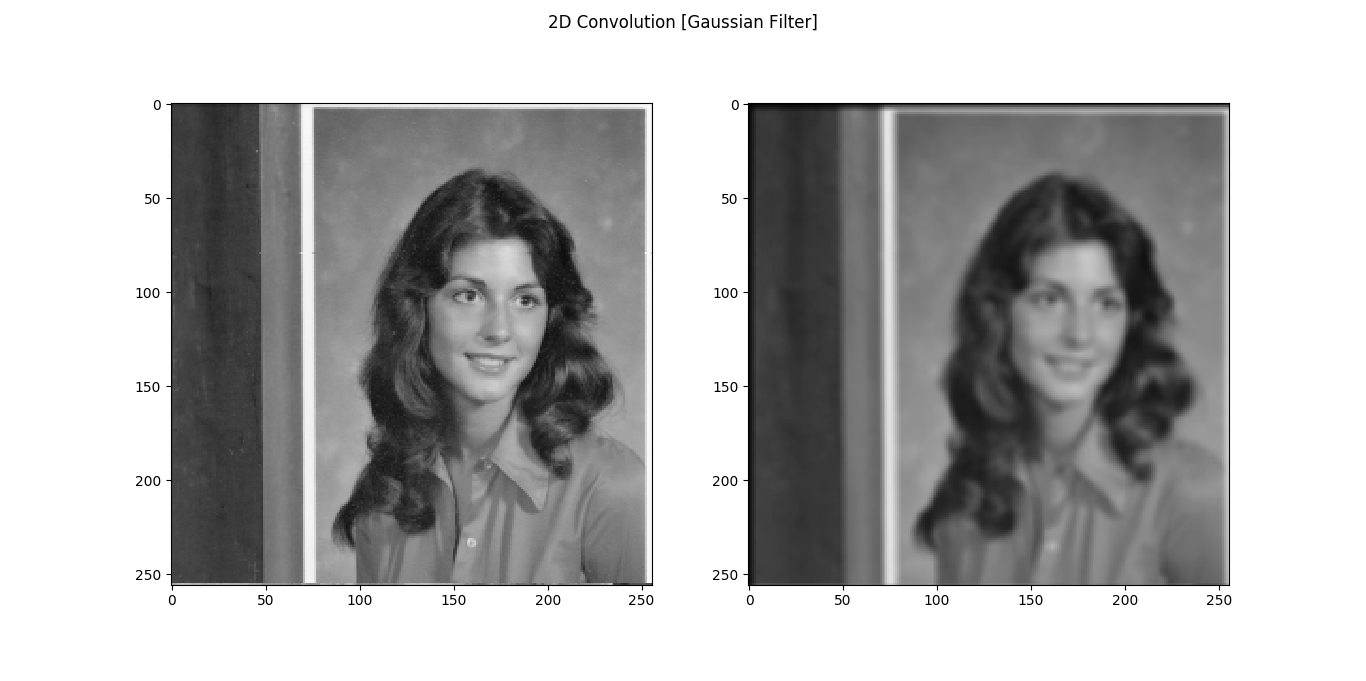
\includegraphics[width=\textwidth]{pics/result.png}
           \captionsetup{justification=centering}
           \captionof{figure}{Результат применения сглаживающего фильтра Гаусса \\
           (\url{https://en.wikipedia.org/wiki/Gaussian_blur}).\\
           Команда для отображения: {\tt python3 ../scripts/plot\_2D.py}}
       \end{figure}
    \end{frame}
    \begin{frame}
        \begin{center}
        \baselineskip 20.0mm
        \Huge Спасибо за внимание!
        \end{center}
    \end{frame}
\end{document}
